\documentclass[a4paper, 16pt]{article}
\usepackage[UTF8]{ctex}
\usepackage{geometry}
\usepackage{graphicx}
\usepackage{setspace}
\usepackage{float}
\usepackage{listings}
\usepackage{xcolor}
\lstset{
    numbers=left, 
    numberstyle= \tiny, 
    keywordstyle= \color{ blue!70},
    commentstyle= \color{red!50!green!50!blue!50}, 
    frame=shadowbox, % 阴影效果
    rulesepcolor= \color{ red!20!green!20!blue!20} ,
    escapeinside=``, % 英文分号中可写入中文
    xleftmargin=2em,xrightmargin=2em, aboveskip=1em,
    framexleftmargin=2em
} 
\geometry{left = 1.0 cm, right = 1.0cm, top = 2.0cm, bottom = 2.0cm	}
\title{编译原理第七章(一)}
\author{李鹏辉}

\begin{document}
\maketitle

1.(7.2.4)下面是两个C语言函数f和g的概述:

int f ( int x ) $\{$ int i; … return i + 1; … $\}$

int g ( int y ) $\{$ int j; … f ( j + 1 ); … $\}$

函数g调用f。画出在g调用f而f即将返回时,运行时刻栈中从g的活动记录开始的顶端部分。你可以只考虑返回值、参数、控制链以及存放局部数据的空间。你不用考虑存放的机器状态,也不用考虑没有在代码中显示的局部值和临时值。但是你应该指出:

1) 哪个函数在栈中为各个元素创建了所使用的空间?

2) 哪个函数写入了各个元素的值? 

3) 这些元素属于哪个活动记录?

\begin{figure}[H]
\centering
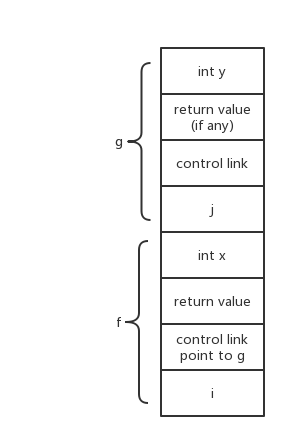
\includegraphics[scale = 0.6]{chapter7_1}
\label{f1}
\end{figure}

每个函数的参数和范围值空间为其调用者创建,函数内部的控制链和局部变量为该函数自己创建。

每个函数的参数,控制链由调用者写入,返回值和临时变量由该函数写入\\

2.(7.3.1):图7-15(见下页)中给出了一个按照非标准方式计算Fibonacci数的ML语言的函数main。函数fib0将计算第n个Fibonacci数(n≥0)。嵌套在fib0中的是fib1,它假设n≥2并计算第n个Fibonacci数。嵌套在fib1中的是fib2,它假设n≥4。请注意,fib1和fib2都不需要检查基本情况。我们考虑从对main的调用开始,直到(对fib0(1)的)第一次调用即将返回的时段,请描述出当时的活动记录栈,并给出栈中的各个活动记录的访问链。
\begin{figure}[H]
\centering
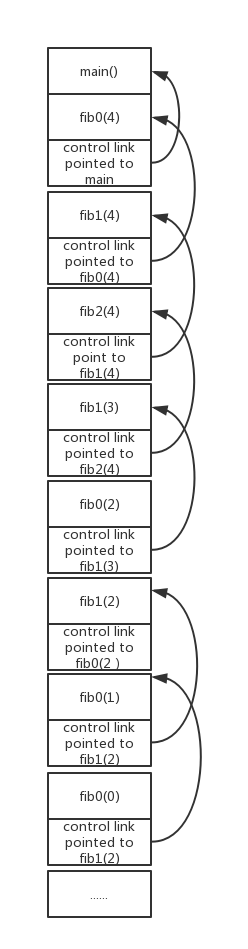
\includegraphics[scale = 0.6]{chapter7_2}
\label{f1}
\end{figure}


3.(7.3.2):假设我们使用display表来实现下图中的函数。请给出fib0(1)的第一次调用即将返回时的display表。同时指明那时在栈中的各个活动记录中保存的display表条目。
\begin{figure}[H]
\centering
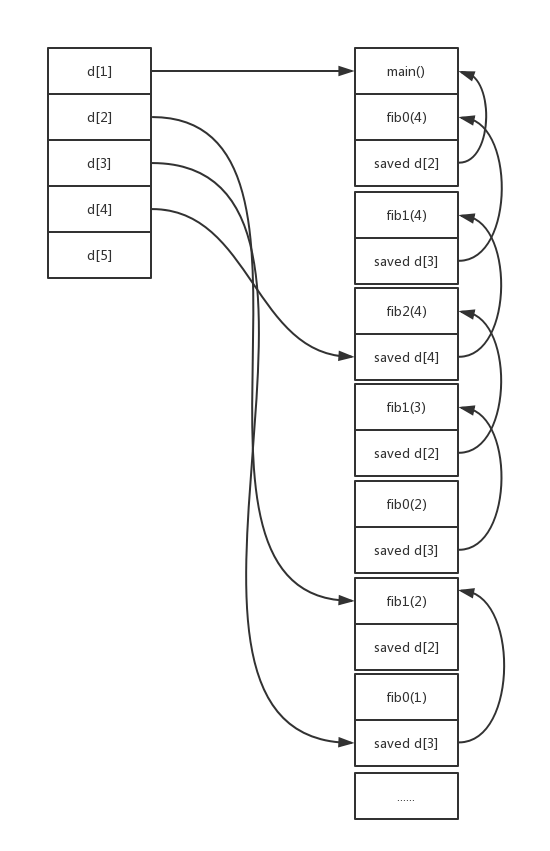
\includegraphics[scale = 0.6]{chapter7_3}
\label{f1}
\end{figure}

\end{document}